\begingroup
	\pgfdeclarelayer{dibujo}
	\pgfsetlayers{dibujo, main}
	\tikzstyle{zero}=[circle,draw=black,fill=gray,inner sep=0pt,minimum size=2.5mm]
	\tikzstyle{one}=[circle,draw=black,fill=black,inner sep=0pt,minimum size=2.5mm]
	\tikzstyle{two}=[circle,draw=black,fill=white,inner sep=0pt,minimum size=2.5mm]
	\tikzstyle{three}=[circle,draw=black,fill=gray!20,inner sep=0pt,minimum size=2.5mm]
	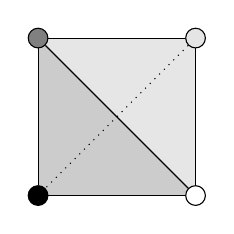
\begin{tikzpicture}
		\node (a) at (-1,1) [zero] {};
		\node (b) at (-1,-1) [one] {};
		\node (c) at (1,-1) [two] {};
		\node (d) at (1,1) [three] {};
		
		\begin{pgfonlayer}{dibujo}
			\filldraw[black,opacity=0.2] (-1,1)--(-1,-1)--(1,-1);
			\filldraw[gray,opacity=0.2] (-1,1)--(1,1)--(1,-1);
		\end{pgfonlayer}
		\draw (d)--(a)--(b)--(c)--(d);
		\draw [dotted] (d)--(b);
		\draw (c)--(a);
	\end{tikzpicture}
	%\label{fig:3_simplex}
\endgroup